\subsection{Why the lead shrinks (E7): results}
\label{sec:ft-why-results}

% E7's results, from FINDINGS section 26 and CLAIMS group H only. Pre-registered, report-only, post-hoc and declared
% exploratory values each say which they are, as their rows do.
\paragraph{The pre-registered outcomes.}
Q3's answer is no for both: the two primaries were equivalent to zero and not superior at $\delta = 0.07$~dB, over all seven scenes with none dropped (Tables~\ref{tab:t4} and~\ref{tab:t4b}, Fig.~\ref{fig:f6}). % s26 "The verdict"; H1, H2
For $\Delta_{\mathrm{refit}}$, $\bar\Delta = -0.0201$~dB with $\mathrm{SE} = 0.00556$, and the equivalence interval $[-0.0332, -0.00694]$~dB lies inside $\pm\delta$. % s26 "Equivalence"; H1
Its superiority test failed on the count alone: 3 of 7 scenes had the mean's sign against the 5 required, while its statistic, 3.61, exceeded the critical value of 2.841. % s26 "Superiority"; H1
For $\Delta_{\mathrm{cb}}$, $\bar\Delta = +0.00844$~dB with $\mathrm{SE} = 0.0111$, and the interval $[-0.0127, +0.0295]$~dB also lies inside $\pm\delta$; Holm's order left its superiority test unrun after $\Delta_{\mathrm{refit}}$'s failure, and its statistic was 0.758 against 2.365. % s26 "Superiority"; H2
The registered reading of these outcomes is that the re-fit does not explain the shrink beyond $\pm\delta$ and that codebook training does not explain the shrink beyond $\pm\delta$. % s26 "The verdict"; H1, H2
Neither primary is fragile: both keep their outcome under the registered BD-level standard error, $\mathrm{SE}_{\mathrm{BD}} = 0.0129$. % s26 "The robustness reading and the fragile flag"; H3

\paragraph{What the outcomes bound.}
Both readings are at equal rate and in the mean over scenes, and the re-fit is of the AC and DC grids together. % s26 "What section 26 settles"; H1, H2
The claim is this bound and not a sign: $\bar\Delta$ is negative for $\Delta_{\mathrm{refit}}$, but $\Delta_{\mathrm{refit}}$ is positive on 4 of 7 scenes and the mean's sign rests on kitchen. % s26 "Post-hoc observations"; H4, H7
The re-fit's effect on the bytes stands (Section~\ref{sec:ac-grid}). % s26 "What section 26 settles"; H1, F9

\paragraph{Against the shrink (post hoc; not an additive split).}
These ratios are outside Q3's answer, which is in dB. % s26 "Post-hoc observations"; H4
In E7's own rows the shrink is P1's 0.354~dB minus P\_FT's 0.0467~dB, which is 0.307~dB, and $\delta$ is 22.8\% of it, about a quarter. % s26 "Post-hoc observations"; H4
The two means are 6.5\% and 2.7\% of the shrink. % s26 "Post-hoc observations"; H4

\paragraph{What neither primary holds fixed (report only and post hoc).}
Nothing in this paragraph is part of Q3's answer. % s26 "What section 26 settles"; H5
Neither primary holds fixed the kept splats' colours, opacity, scaling, the scaling factor or rotation; positions have a learning rate of 0 and do not train. % s24 item 4; s26 "What section 26 settles"; H5
Report only: $\mathrm{BD}_K - \mathrm{BD}_R$ has mean 0.255~dB and $\mathrm{BD}_K - \mathrm{BD}_{CG}$ mean 0.266~dB, each positive on all seven scenes (Table~\ref{tab:t5}). % s26 "Secondaries"; H5
Post hoc, measured from P1: under arm K, where only the codewords train, the lead shrinks by only 17.2\% of the full shrink; under arm CG, where everything but the codewords trains, by 103.8\% of it (per-arm curves on two scenes in Fig.~\ref{fig:f7}). % s26 "Post-hoc observations"; H5
So the shrink is carried mostly by fine-tuning the parameters outside the grids and the codebook, the case the registered reading of two equivalent primaries describes. % s26 "The verdict"; H5
These are interventions and not an additive split, and E7 has no arm that separates those parameters from one another, so it does not say which of them carries the shrink. % s26 "What section 26 settles"; H5

\paragraph{Robustness.}
Beyond $\mathrm{SE}_{\mathrm{BD}}$, two post-hoc, undeclared standard errors at 6 degrees of freedom give the same outcomes, and neither replaces the registered SE. % s26 "Post-hoc observations"; H8
With the replicate pair's spread across scenes, $\mathrm{SE} = 0.0128$ for both primaries and the equivalence margins are $m = 3.89$ for $\Delta_{\mathrm{refit}}$ and $m = 4.79$ for $\Delta_{\mathrm{cb}}$. % s26 "Post-hoc observations"; H8
With the scene spread of $\Delta_s$, $\mathrm{SE} = 0.0227$ for $\Delta_{\mathrm{refit}}$ and 0.0124 for $\Delta_{\mathrm{cb}}$, and $\Delta_{\mathrm{cb}}$ comes first in Holm's order ($m = 4.97$). % s26 "Post-hoc observations"; H8
$\Delta_{\mathrm{refit}}$'s equivalence ($m = 2.20$) holds at its Holm position, second, with critical $t$ 1.943, though it would not clear the first position's critical value, 2.447. % s26 "Post-hoc observations"; H8
Exploratory and declared before unblinding, leaving drjohnson's $j = 0$ seed pair out of the noise pooling ($\mathrm{SE} = 0.00598$ and 0.0118, six degrees of freedom) changes neither outcome; the verdict is the pre-registered computation. % s26 "Exploratory sensitivity"; H6
Kitchen is the only scene beyond $\pm\delta$, at $\Delta_{\mathrm{refit}} = -0.150$~dB, and the other 6 scenes average $+0.00158$~dB (post hoc); why it stands apart is not settled. % s26 "Post-hoc observations"; H7

\paragraph{Discussion: fine-tuning and the starting quantiser.}
That fine-tuning with the quantiser in the loop removes most of the difference between two starting quantisers is known from neural-network quantisation.
Nagel et al.\ report that ResNet18 with 4-bit weights and 8-bit activations reached 0.12\% ImageNet accuracy after post-training quantisation from a min-max weight grid and 18.58\% from an MSE-fitted grid, but 69.61\% and 69.76\% after quantisation-aware training from the same two grids; these numbers are quoted from the source \citep[Table~8]{nagel2021white}. % quoted nagel2021white (Table 8, p. 22)
Xu et al.\ trace the weakness of post-training quantisation at very low precision to a misalignment between the local, layer-wise error it minimises and the global loss that quantisation-aware fine-tuning minimises \citep{xu2025understanding}.
E7's outcome is of the same kind: OGC's VQ led by 0.3558~dB before C3DGS's fine-tuning and by 0.0425~dB after it, and neither the colour grids' re-fit nor codebook training explains the shrink beyond $\pm\delta$. % s19 "The verdict"; s21 "The verdict"; s26 "The verdict"; A2, F1, H1, H2
The same literature marks where the erasure stops: at 2 bits the starting point still matters after fine-tuning, which LoftQ and ApiQ address by initialising low-rank fine-tuning jointly with the quantised weights \citep{li2024loftq,liao2024apiq}, and EfficientQAT's 2-bit Llama-2-70B still trails full precision after quantisation-aware training, 69.48 against 72.41 in the source's accuracy measure (quoted from the source) \citep{chen2025efficientqat}. % quoted chen2025efficientqat (abstract)
So the erasure E7 found is what this literature leads one to expect at moderate precision, the regime of C3DGS's 4,096-entry codebook and 8-bit grids, and it may not hold at very low rates or with much smaller codebooks (Section~\ref{sec:limits}). % s26 "The verdict"; H1, H2

\paragraph{Two session facts.}
Drjohnson's $j = 0$ seed pair spans two Kaggle images and is reported as spanning under Note~2 C6.\footnote{\sloppy S3 ran on \code{py3.13.15|\allowbreak torch2.11.0+cu128|\allowbreak cuda12.8|\allowbreak cudnn91900|\allowbreak driver580.178.04} and S11 on \code{py3.13.16|\allowbreak torch2.11.0+cu130|\allowbreak cuda13.0|\allowbreak cudnn92700|\allowbreak driver580.178.04}.} % s26 "How the sessions ran"; H13
S10's restore ran before four of its bundle datasets were attached, with no data effect: every copy it restored is byte-identical to its S9 reference copy. % s26 "How the sessions ran"; H13

\begin{table}[t]
\centering
\footnotesize
\caption{E7 per scene (BD-PSNR, dB, 6 decimals): each arm's BD from its seed-0 curve and the two pre-registered primaries, with $\bar\Delta$, $\mathrm{SD}_{\mathrm{pool}}$ and SE in the footer. Generated from the committed bundles.} % s26 "The primaries per scene"; H1, H2
\label{tab:t4}
% Amendment 20 f: BD per arm and the two primaries (bench/gn/e7.py)
% generated by paper/figs/e7_t4_primaries.py from E7's bundles (bench/gn/e7.py); do not edit
\begin{tabular}{lrrrrr}
\toprule
Scene & BD\_R & BD\_G & BD\_CG & $\Delta_{\mathrm{refit}}$ & $\Delta_{\mathrm{cb}}$ \\
\midrule
bonsai & +0.073025 & +0.081185 & +0.127371 & +0.008160 & +0.046187 \\
counter & +0.081245 & +0.050226 & +0.076107 & -0.031020 & +0.025882 \\
drjohnson & -0.009510 & +0.016630 & -0.018900 & +0.026139 & -0.035530 \\
kitchen & +0.041541 & -0.108538 & -0.065459 & -0.150079 & +0.043079 \\
playroom & +0.066940 & +0.058966 & +0.056049 & -0.007974 & -0.002916 \\
room & +0.042699 & +0.052854 & +0.064884 & +0.010155 & +0.012030 \\
truck & +0.031003 & +0.035014 & +0.005348 & +0.004011 & -0.029666 \\
\midrule
$\bar\Delta$ &  &  &  & -0.020087 & +0.008438 \\
SD\_pool &  &  &  & 0.014715 & 0.029460 \\
SE = SD\_pool / $\sqrt{n}$ &  &  &  & 0.005562 & 0.011135 \\
\bottomrule
\end{tabular}

\end{table}

\begin{table}[t]
\centering
\footnotesize
\caption{E7's tests, Holm-corrected per test type: the position, the statistic ($|\bar\Delta| / \mathrm{SE}$ for superiority, the margin $m$ for equivalence), the critical $t$ and the result; then each primary's outcome under SE, the one of record, and under $\mathrm{SE}_{\mathrm{BD}}$. Generated from the committed bundles.} % s26 "Superiority", "Equivalence"; H1, H2, H3
\label{tab:t4b}
% Amendment 20 f, h: Holm-ordered tests, outcomes, robustness (delta = 0.07 dB; n = 7)
% generated by paper/figs/e7_t4_primaries.py from E7's bundles (bench/gn/e7.py); do not edit
\begin{tabular}{llrrrl}
\toprule
Primary & Test & Holm position & Statistic & Critical t & Result \\
\midrule
refit & superiority & 1 & 3.612 & 2.841 & not superior \\
refit & equivalence & 1 & 8.975 & 2.365 & equivalent \\
refit & outcome (SE) &  &  &  & equivalent; not superior \\
refit & outcome (SE\_BD) &  &  &  & equivalent; not superior \\
cb & superiority & 2 & 0.758 & 2.365 & not tested (Holm) \\
cb & equivalence & 2 & 5.529 & 1.895 & equivalent \\
cb & outcome (SE) &  &  &  & equivalent; not superior \\
cb & outcome (SE\_BD) &  &  &  & equivalent; not superior \\
\bottomrule
\end{tabular}

\end{table}

\begin{table}[t]
\centering
\scriptsize
\setlength{\tabcolsep}{3pt}
\caption{E7's secondaries per scene (dB; report only, no bars): the arm differences, P1 with each method's own grid against P1, P\_FT and P1 from the seed-0 (s0) and seed-1 (s1) curves, and the replicate pair at $j = 0$. Generated from the committed bundles.} % s26 "Secondaries"; H5, H9, H10, H11
\label{tab:t5}
% Amendment 20 g: secondaries, report only (bench/gn/e7.py)
% generated by paper/figs/e7_t5_secondaries.py from E7's bundles (bench/gn/e7.py); do not edit
\begin{tabular}{lrrrrrrrrr}
\toprule
Scene & K - CG & K - R & O - G & P1\_own - P1 & P\_FT s0 & P\_FT s1 & P1 s0 & P1 s1 & Replicate \\
\midrule
bonsai & +0.2783 & +0.3327 & +0.0070 & +0.0595 & +0.0730 & +0.0211 & +0.4811 & +0.4867 & +0.0419 \\
counter & +0.2165 & +0.2114 & +0.0409 & +0.1124 & +0.0812 & +0.1161 & +0.3193 & +0.3339 & +0.0177 \\
drjohnson & +0.2384 & +0.2290 & -0.0361 & +0.0202 & -0.0095 & +0.0043 & +0.2757 & +0.2960 & -0.0578 \\
kitchen & +0.4158 & +0.3088 & +0.0959 & +0.0725 & +0.0415 & +0.0830 & +0.4008 & +0.4224 & -0.0116 \\
playroom & +0.2909 & +0.2800 & +0.0190 & +0.0016 & +0.0669 & +0.0223 & +0.4629 & +0.4678 & -0.0417 \\
room & +0.2925 & +0.3146 & -0.0142 & +0.0522 & +0.0427 & +0.0347 & +0.3894 & +0.3956 & -0.0107 \\
truck & +0.1311 & +0.1055 & -0.0103 & +0.0292 & +0.0310 & +0.0126 & +0.1487 & +0.1573 & -0.0248 \\
\midrule
mean & +0.2662 & +0.2546 & +0.0146 & +0.0497 &  &  &  &  &  \\
SE = SD\_pool / $\sqrt{n}$ & 0.0142 & 0.0099 & 0.0099 &  &  &  &  &  &  \\
SD\_BD (scenes used) &  &  &  &  & 0.0242 (7) &  & 0.0095 (7) &  &  \\
SD across scenes &  &  &  &  &  &  &  &  & 0.0340 \\
\bottomrule
\end{tabular}

\end{table}

\begin{figure}[t]
\centering
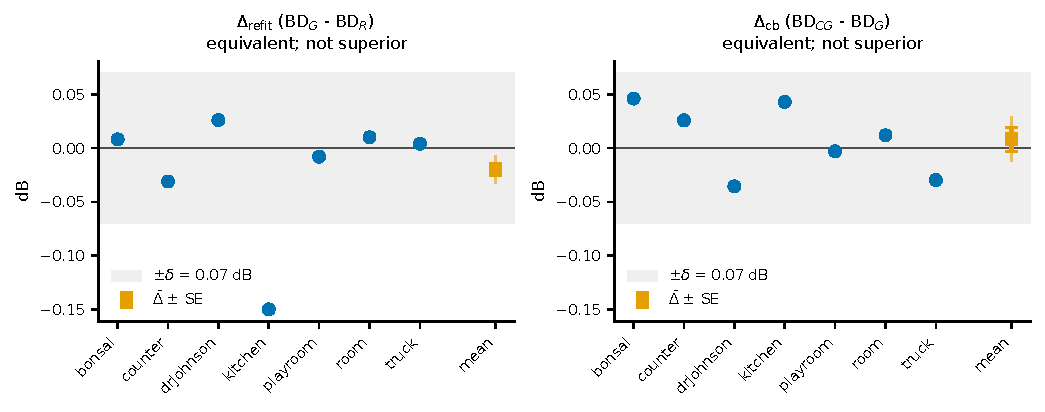
\includegraphics[width=\linewidth]{e7_f6_deltas.pdf}
\caption{E7's primaries per scene. Each circle is a scene's $\Delta_s$. The square is $\bar\Delta$ with a bar of $\pm$SE, and the lighter bar is $\pm$ the critical $t$ of its Holm position times SE. The shaded band is $\pm\delta$, and each title carries the registered outcome.} % s26 "The primaries per scene"; H1, H2, H7
\label{fig:f6}
\end{figure}

\begin{figure}[t]
\centering
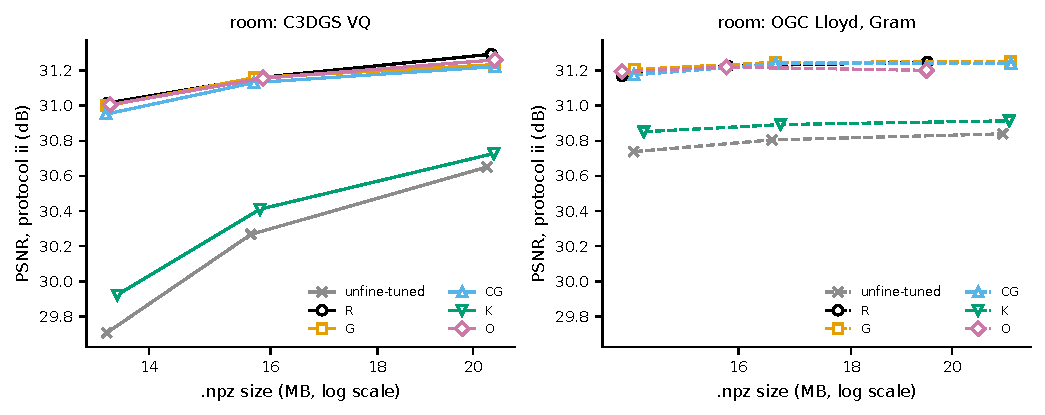
\includegraphics[width=\linewidth]{e7_f7_arm_curves_room.pdf}
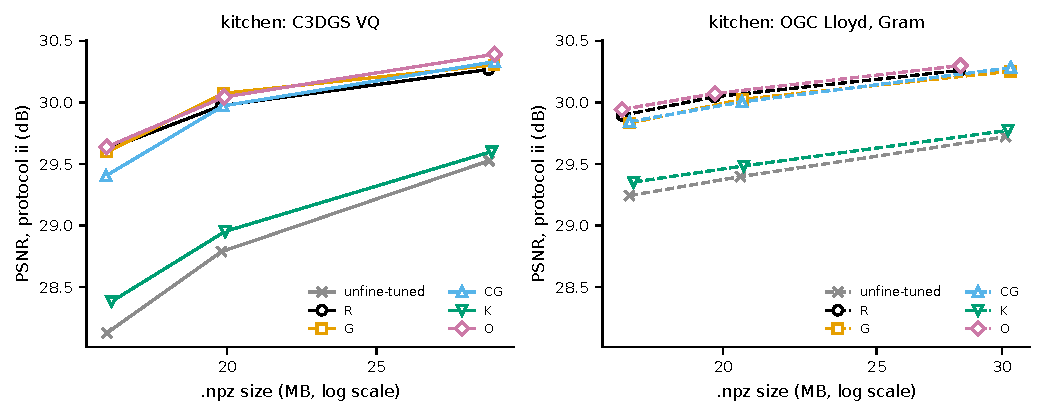
\includegraphics[width=\linewidth]{e7_f7_arm_curves_kitchen.pdf}
\caption{Each arm's fine-tuned curve for each method on room (top) and on kitchen (bottom), the one scene beyond $\pm\delta$, with the unfine-tuned row for reference: protocol~ii PSNR against \code{.npz} size, seed 0, one process per point. On each scene the two panels share the PSNR axis.} % s26 "Secondaries"; H5, H7
\label{fig:f7}
\end{figure}
